%Copyright 2014 Jean-Philippe Eisenbarth
%This program is free software: you can 
%redistribute it and/or modify it under the terms of the GNU General Public 
%License as published by the Free Software Foundation, either version 3 of the 
%License, or (at your option) any later version.
%This program is distributed in the hope that it will be useful,but WITHOUT ANY 
%WARRANTY; without even the implied warranty of MERCHANTABILITY or FITNESS FOR A 
%PARTICULAR PURPOSE. See the GNU General Public License for more details.
%You should have received a copy of the GNU General Public License along with 
%this program.  If not, see <http://www.gnu.org/licenses/>.

%Based on the code of Yiannis Lazarides
%http://tex.stackexchange.com/questions/42602/software-requirements-specification-with-latex
%http://tex.stackexchange.com/users/963/yiannis-lazarides
%Also based on the template of Karl E. Wiegers
%http://www.se.rit.edu/~emad/teaching/slides/srs_template_sep14.pdf
%http://karlwiegers.com
\documentclass{scrreprt}
\usepackage{listings}
\usepackage{underscore}
\usepackage[bookmarks=true]{hyperref}
\usepackage[utf8]{inputenc}
\usepackage[english]{babel}
\usepackage[pdftex]{graphicx}
\hypersetup{ bookmarks=false,    % show bookmarks bar?  pdftitle={Software Requirement Specification},    % title
  pdfauthor={Michael Vessia Jr.},                     % author
  pdfsubject={Requirements for GNAT},                        % subject of the document
  pdfkeywords={Networks, Testing, GNAT}, % list of keywords
  colorlinks=true,       % false: boxed links; true: colored links
  linkcolor=blue,       % color of internal links
  citecolor=black,       % color of links to bibliography
  filecolor=black,        % color of file links
  urlcolor=purple,        % color of external links
  linktoc=page            % only page is linked
}%
\def\version{1.0}
\def\sourcecode{https://github.com/MichaelVessia/gnat}
\def\railssource{https://github.com/MichaelVessia/gnat-rails}
\def\author{Michael Vessia Jr.}
\date{}
%\title
\usepackage{hyperref}
\begin{document}

\begin{flushright}
  \rule{16cm}{5pt}\vskip1cm
  \begin{bfseries}
    \Huge{SOFTWARE REQUIREMENTS\\ SPECIFICATION}\\
    \vspace{1.9cm}
    for\\
    \vspace{1.9cm}
    General Network Access Tester\\
    \vspace{1.9cm}
    \LARGE{Version \version}\\
    \vspace{1.9cm}
    Prepared by \author\\
    \vspace{1.9cm}
    \today\\
  \end{bfseries}
\end{flushright}

\tableofcontents

\chapter{Introduction}

\section{Purpose}

General Network Access Tester is an Android application which helps IT departments, network administrators, or anyone that wants to monitor a network that they have access to. The application should be free to download on the Google Play store, and the application will be open source. The application provides information that will make it easier for someone to troubleshoot their network.  The application also reduces the workload on IT departments by allowing them to troubleshoot more quickly.

This document is meant to give an overview of the features of the General Network Access Tester, making the process of using the application for one's own network simple, and making contributing to the project easy and painless.

\section{Document Conventions}
The General Network Access Tester will hereafter be referred to as GNAT\@. Users will be someone that interacts with the mobile application.  An administrator will be the person who owns the network and is likely having the logs sent to them.  The administrator can and likely will also be the user.

\section{Intended Audience and Reading Suggestions}
This document is meant for administrators who would like to have their network monitored by GNAT, or developers who would like to make contributions to GNAT\@. It is not required that users read this document, but if they would like further clarification about the settings they they are configuring within the application, they will find that information in this document.  Developers will be interested in the source code. As of version \version, the source code can be found at \sourcecode.

\section{Project Scope}

GNAT is targetting network administrators who have mobile devices connecting to their network and would like more information about connection attempts, connection drops, and other network issues. It should reduce the time an IT team needs to troubleshoot why people are unable to connect to their network.

\chapter{Overall Description}

\section{Product Perspective}

GNAT should integrate well with third party software as the logs are in JSON format, but ultimately should be a stand-alone application and not depend on any other software. More functionality is unlocked if the administrator has a server that accepts JSON POST requests.

GNAT's output log files should integrate well into an existing monitoring/dashboard system, but this is not required for the application to function.


\section{Product Functions}


Within the mobile application, users will be able to enter a number of configuration options that will affect what kind of logs are generated. The connection info will be logged in the background at a user specified interval. Although the application tests network access, it ultimately assumes that the user has access to the internet.  If there is no wifi network to connect to, functionality will be extremely limited.

The application needs internet (WIFI) to generate the desired logs and send them to the server. 

If the administrator uses a dashboard service that has an API, it should accept JSON POST requests, and they can enter the url into GNAT's settings.  If it does not, they are responsible for creating some kind of web service that can act as a middle man.

\section{User Classes and Characteristics}
The user of the application is expected to either be the administrator, or be a knowledgeable user that recieved the relevant information from the administator.  End users of the network should not have to interact with GNAT, but assuming they had the relevant information nothing would be stopping them.

\section{Operating Environment}
GNAT will run on the Android operating system.  The application will require the user to have at least Android 4.0.3 (Ice Cream Sandwich). It also assumes there is a network to be tested.

Outside of the application, the administrator should feel free to create an internet facing web page, and place a file on that page.  The app will attempt to connect to this web page, based on the address the user enters in the configuration. GNAT can simply check if the file was able to be downloaded, or the file can be a script that does something else and stores more detailed logs on the server.

\section{Design and Implementation Constraints}

\begin{itemize}
\item GNAT will write JSON logs to local device storage, there should be room on the device. It will not delete any old logs, this is up to the user.
  \item GNAT will send POST requests to the server specified.  This server needs to be properly configured and must exist.
\end{itemize}

\section{Assumptions and Dependencies}

\begin{itemize}
\item If a user plans to use a third party monitoring system, they need to make sure they are credentialed to do so and that the service provides an API\@. If the service has not yet been used with GNAT, a user should feel free to add their anonymized script to the repository, and create a pull request at \sourcecode.
\item GNAT assumes the user knows the password to the network they are trying to test.  Failure to connect should be from other issues, not authentication.
\end{itemize}

\chapter{External Interface Requirements}

\section{User Interfaces}

\begin{center}
  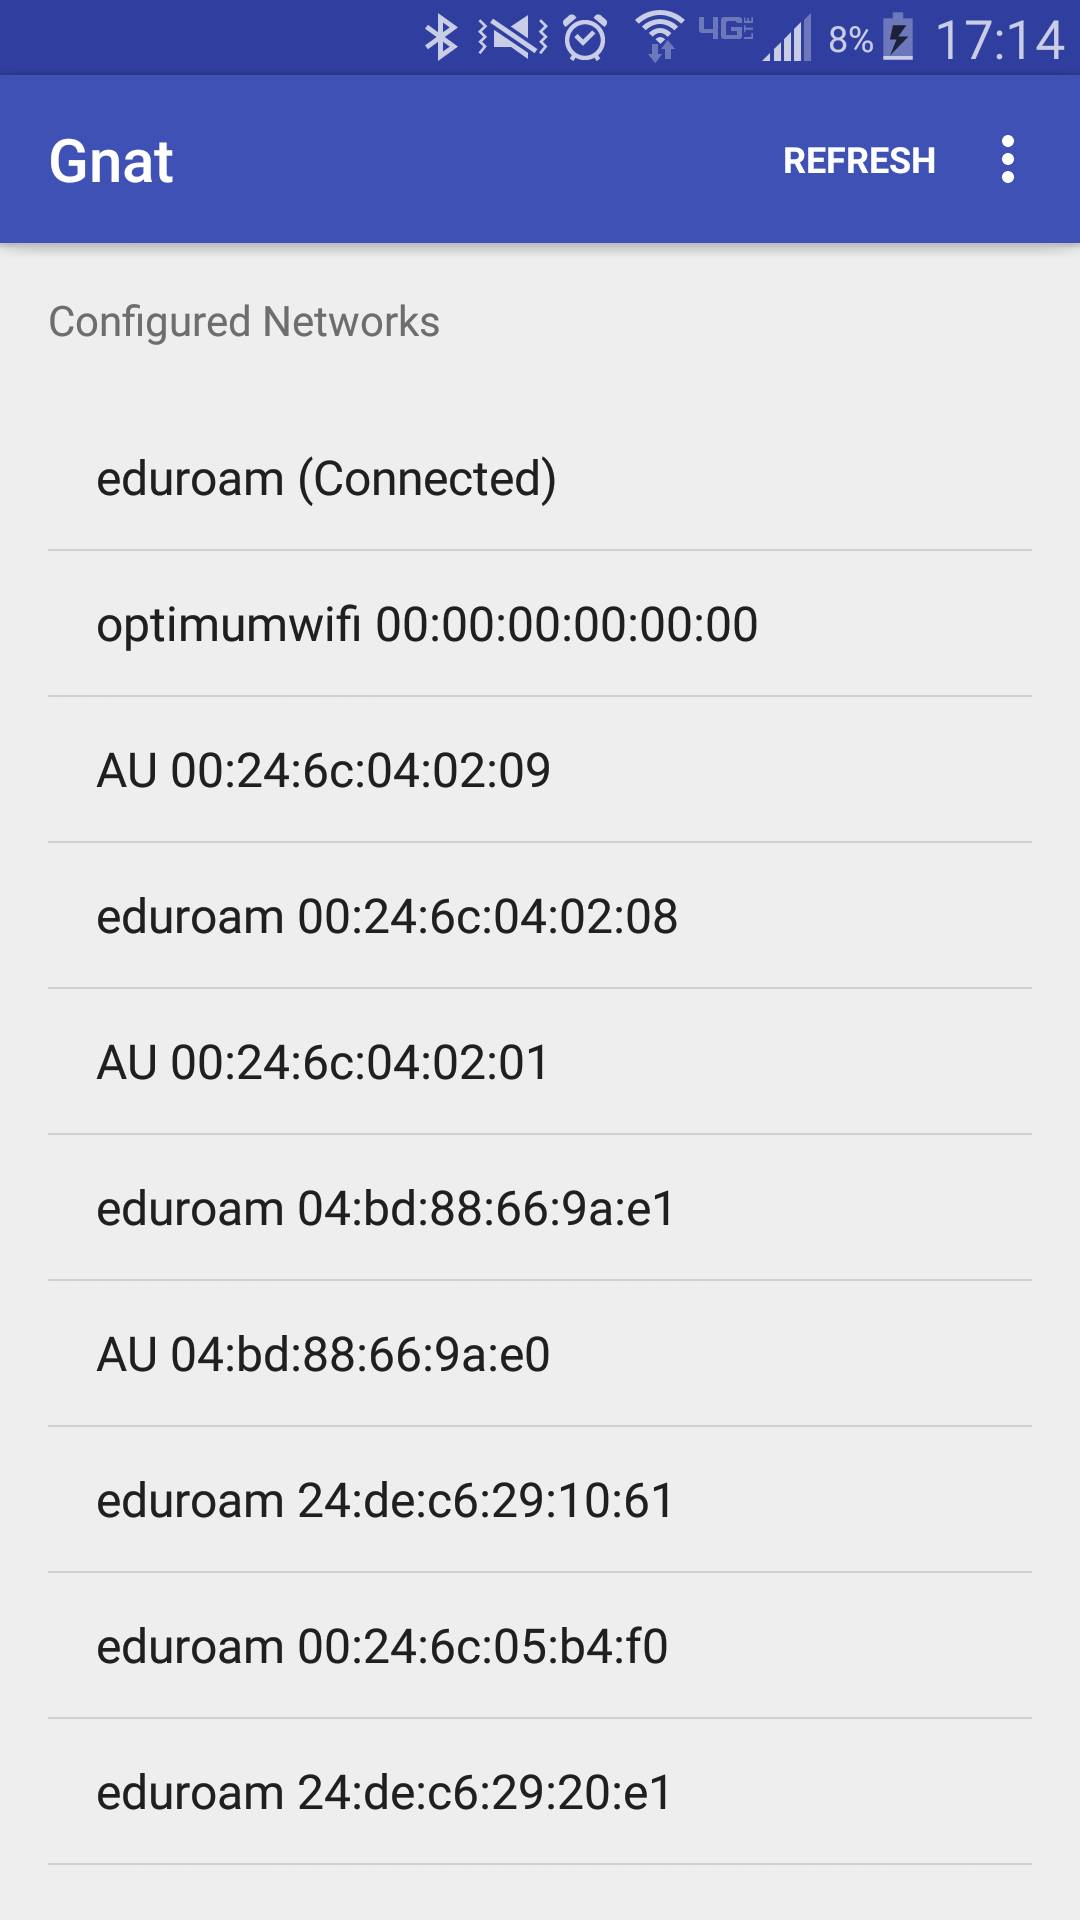
\includegraphics[scale=0.3]{mainActivity.jpg}

  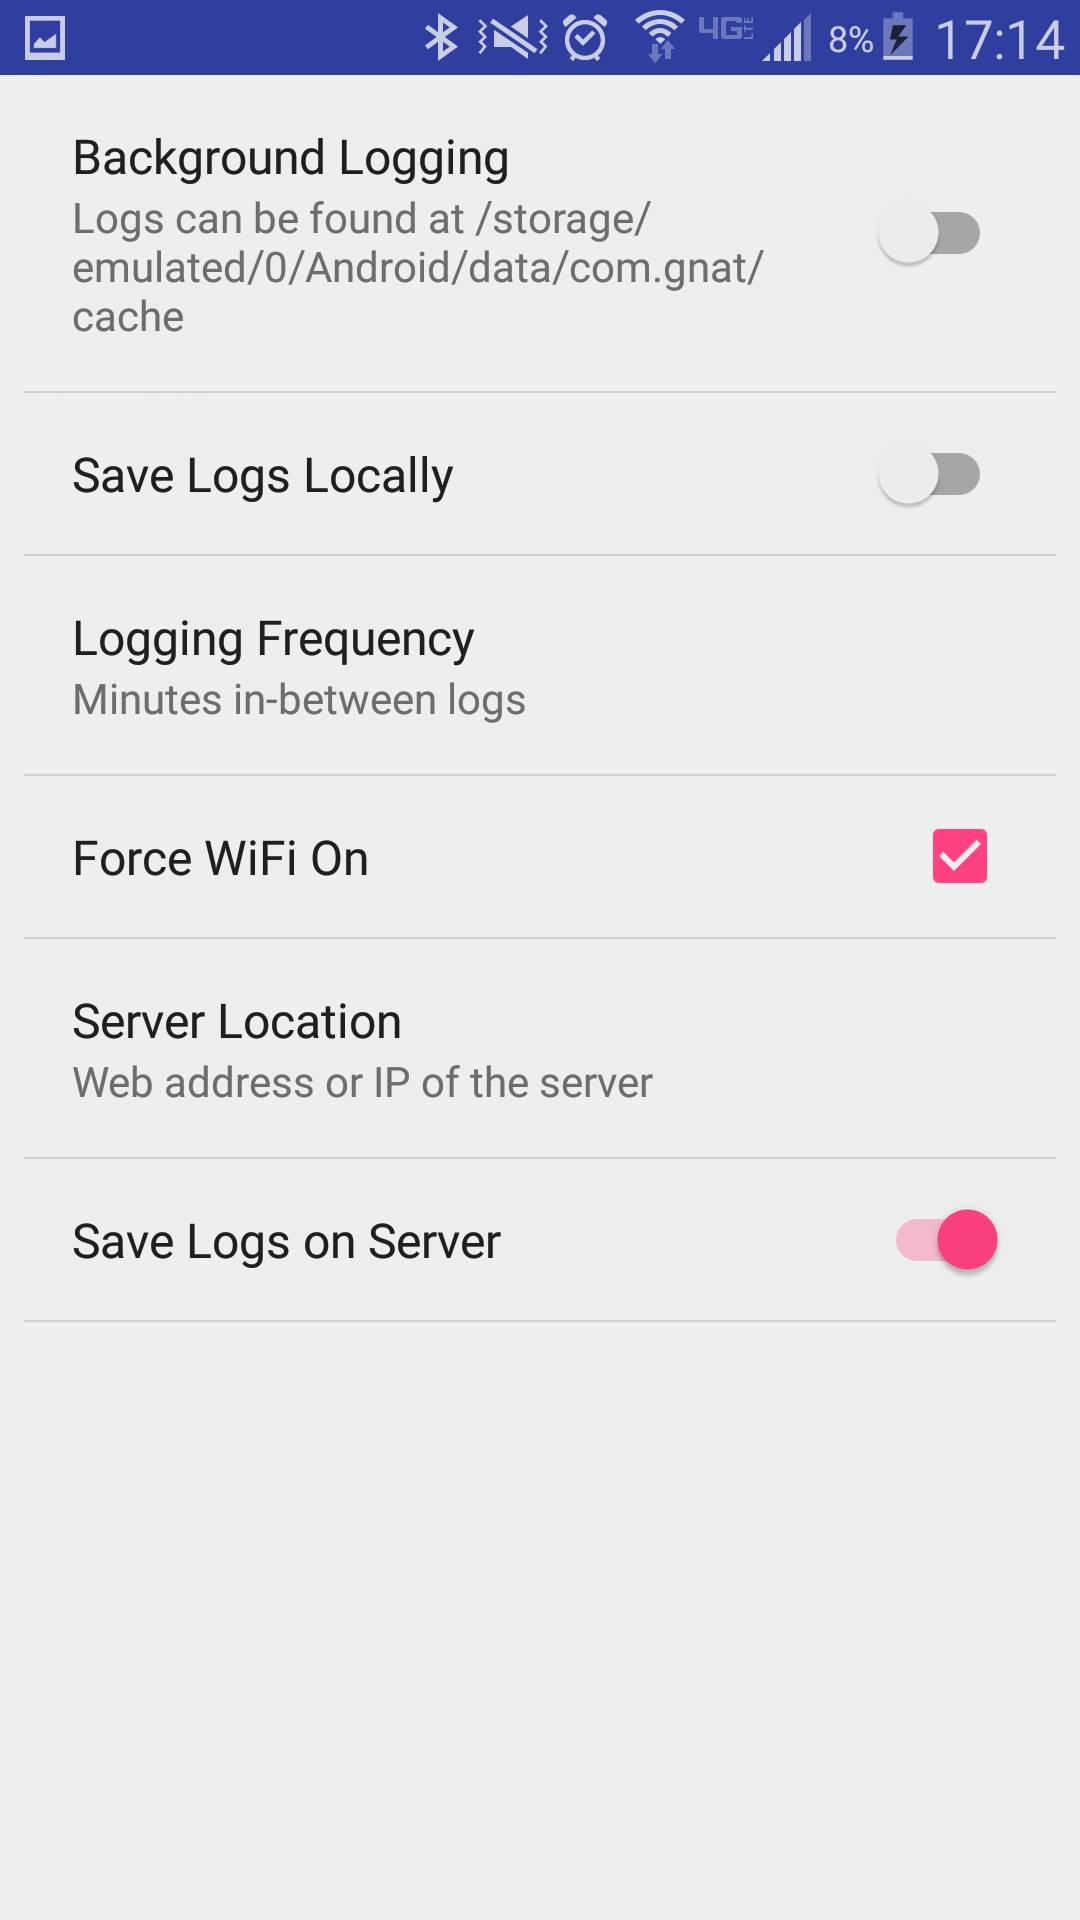
\includegraphics[scale=0.3]{settings.jpg}
  \end{center}

\section{Software Interfaces}

A sample web app for companion use with GNAT exists at \railssource.  It was built with Ruby on Rails and PostgreSQL.  Administrators should feel free to create their own using their own server/technology stack.

\section{Communications Interfaces}

Logs are sent via HTTP POST request using the application/json header.

\chapter{System Features}

\section{Generation of Log Files}

\subsection{Description and Priority}

Priority: High

Necessary for the desired purpose of the application.  Without the log files, GNAT's use is limited.

\subsection{Stimulus/Response Sequences}
\begin{enumerate}
\item User connects to the network
\item User enters configuration, enables logging
\item Log file is generated at specified interval
\end{enumerate}

\subsection{Functional Requirements}

\begin{itemize}
\item Log Files should be in JSON format to make the integration with APIs easier in the future.
\end{itemize}

\section{Connection to Administrator's Server}

\subsection{Description and Priority}

Priority: High

If there is no web page to connect to, then we can only monitor connection failure and nothing beyond that. Having a server with a web page allows us to offload log storage onto the server as well.

\subsection{Stimulus/Response Sequences}

\begin{enumerate}
  \item User enters appropriate configuration options and begins logging.
\item JSON object is generated containing log information.
  \item HTTP POST request is made to server.
\end{enumerate}

\subsection{Functional Requirements}

\begin{itemize}
\item Log files are stored on the server
\item Log files should be sent through an API to the IT monitoring software if it is provided
\item If a network connection is unable to be established, log files should be stored locally
\end{itemize}

\section{Software Quality Attributes}
One of GNAT's key goals is to be useful to anyone, regardless of their network configuration or external software that they use.  For this reason, it is necessary that it remain open source so that if someone wants to make it useable for their system, they can implement the necessary changes to do so.

\section{Appendix A:\@ Glossary}
\textbf{GNAT}: General Network Access Tester\\
\textbf{HTTP}: Hypertext Transfer Protocol\\
\textbf{HTTPS}: Hypertext Transfer Protocol Secure\\
\textbf{API}: Application Program Interface\\
\textbf{JSON}: JavaScript Object Notation\\
\textbf{XML}: eXtensible Markup Language\\
\textbf{app}: Application\\
\textbf{OS}: Operating System\\
\end{document}










